\chapter{Numerical experiments}

In this section the results of numerical experiments should be placed.
They can confirm or contradict the expectation from the previous sections. 
The forms of result presentation are plots, tables, histograms, pictures, etc.
\begin{enumerate}
    \item Enumerating languages and programs used in the research.
    \item Describing in detail data sets you used.
    \item Presenting the metrics used.
    \item Presenting the results achieved in the experiment.
    \item Comparing the results of the experiment with those obtained using other methods.
    \item Outlining the benefits of the used method.
\end{enumerate}

\begin{table}[!htb]
    \centering
     \caption{
     The description of the table. Highlighting the main point following from this table.}
    \begin{tabular}{cccc}
    \toprule
         & Method 1 & Method 2 & Method 3  \\
        \midrule
      Metric 1   & $\mathbf{10}$ & $20$  & $30$ \\
      Metric 2   & $0.9$ & $0.4$ & $\mathbf{0.1}$ \\
      \bottomrule
    \end{tabular}
    \label{tab::methods_metrics}
\end{table}

Main requirements to plots:
\begin{itemize}
    \item sufficiently large font size for legend, axis labels, axis ticks;
    \item proper scale of y-axis: linear or logarithmic;
    \item clear difference in the rendering of lines corresponding to different methods.
\end{itemize}
\begin{figure}[!htb]
    \centering
    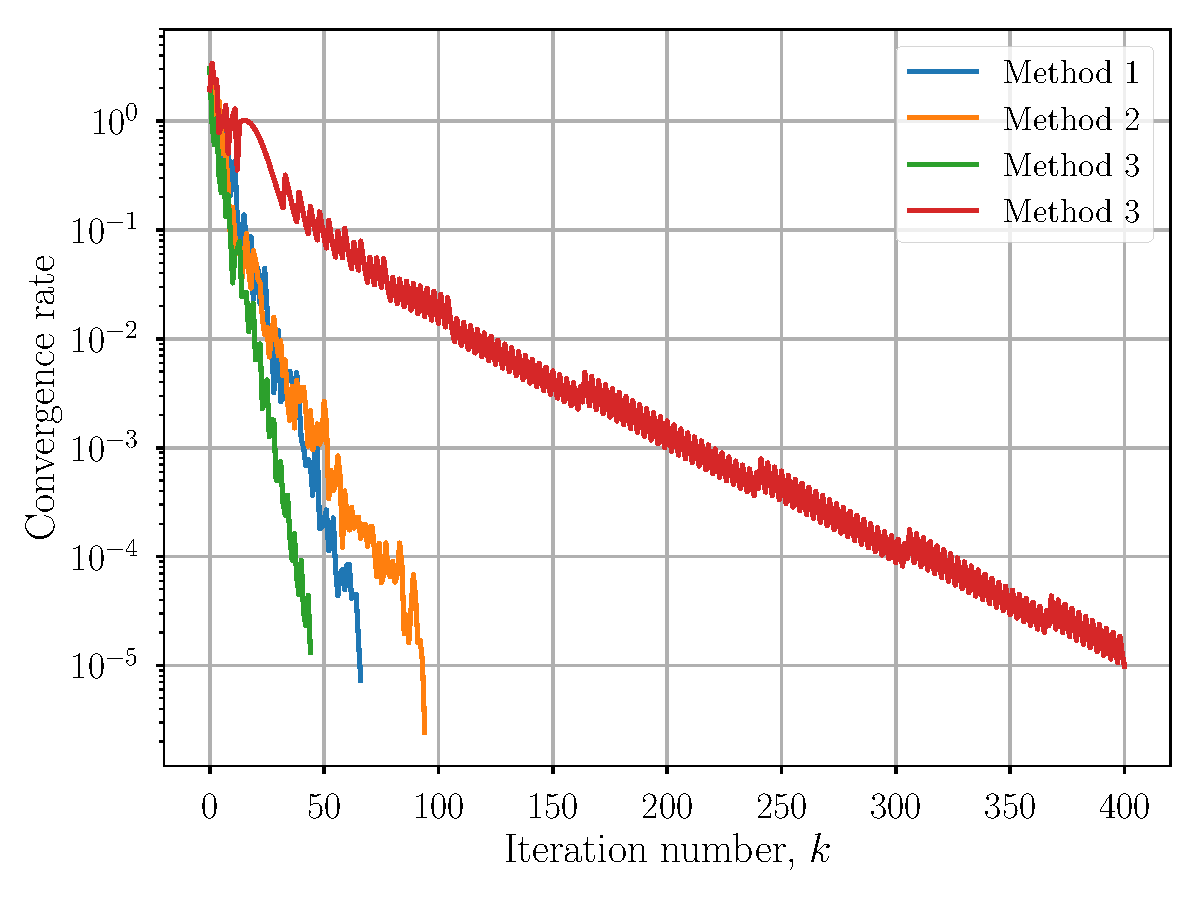
\includegraphics[width=0.4\textwidth]{images/test_plot.pdf}
    \caption{Comparison of the considered methods}
    \label{fig::x_vs_y}
\end{figure}


